\chapter{Motivation}\label{ch:motivation}
This chapter accounts for the motivation behind source signal recovery from electroencephalography (EEG) measurements. The concept of EEG is introduced along with current applications. The potential and importance of source recovery are considered and is related to the hearing aid industry. A commonly applied mathematical model for EEG measurements is presented. Currently applied methods for source recovery are considered leading to a presentation of the current state of the art methods which succeed to overcome the limitations of previous methods. Lastly, the objective of this thesis is specified.          

%%This chapter examines existing literature concerning source recovery from Electroencephalography (EEG) measurements. 
%%At first a motivation for the source recovery problem is given, considering the application within the hearing aid industry. 
%%Further, the state of the art methods are presented followed by a description of the contribution proposed in this thesis.

\section{Introduction to EEG Measurements}\label{sec:EEG}
EEG is an imaging technique used within the medical field. EEG measures electric signals on the scalp, caused by brain activity. 
The human central nerve system consists of various nerve cells connecting the neurons within the brain. Nerve cells respond to certain stimuli, for instance a physical stimulus, and transmit informations between neurons.
Generally speaking these activities induce local currents that are transferred throughout the nerve system. 
Several nearby simultaneous activations result in local potential fields, each referred to as one source signal \cite{EEGsignalprocessing}. 
EEG measurements are provided by a number of metal electrodes, referred to as sensors, carefully placed on the human scalp. 
Each sensor captures the present electrical signals over time.
For the source signal to reach a sensor it has to penetrate the skull, skin and several other thin layers of biological tissue. 
This causes an unknown distortion and reduction of a signal.
It is most likely that the measurements of one sensor are sums of multiple source signals from different areas of the brain.
Furthermore, the range of a single sensor is not separated from the other sensors. 
Thus the same source signal can easily be measured by two or more sensors.
The process of distortion and mixing of signals is called volume conduction \cite{EEGsignalprocessing}\cite{Van2019}. 
The concept of volume conduction is sought illustrated in figure \ref{fig:volumeconduction}.
From this it is clarified that EEG measurements are a mixture of fluctuating electrical signals originating from brain activities. Due to this mixing and the nature of the source signals, the true number of sources are in general considered unknown \cite{EEGsignalprocessing}. 
Furthermore, EEG is a subject for interfering noise. Noise signals can occur in the measurements resulting from physical movement of e.g. eyes and jawbone \cite{fundamentalEEG}.

The source signals are classified within four groups according to the dominant frequency. 
The delta wave ($0.5-4$ Hz) is observed from deep sleep, the theta wave ($4-8$ Hz) is observed from consciousness slips towards drowsiness, the alpha wave ($8-13$ Hz) is the most extensive studied brain rhythm, which is induced by an adult laying down with closed eyes. 
Lastly, the beta wave ($13-30$ Hz) is considered the normal brain wave for adults, associated with active thinking, active attention or solving concrete problems \cite[p. 10]{EEGsignalprocessing}. 
An example of signals within the four categories is illustrated by figure \ref{fig:EEG_example}. 

Generally, the distribution of EEG measurements of multiple sensors is considered multivariant Gaussian \cite[p. 50]{EEGsignalprocessing}. Though the mean and covariance properties generally changes over time. Therefore, EEG measurements are considered quasi-stationary i.e. stationary only within small intervals. This motivates the need for segmentation of the EEG measurements to achieve signals with similar characteristics. 
\begin{figure}[H]
    \begin{minipage}[t]{.45\textwidth}
        \centering
        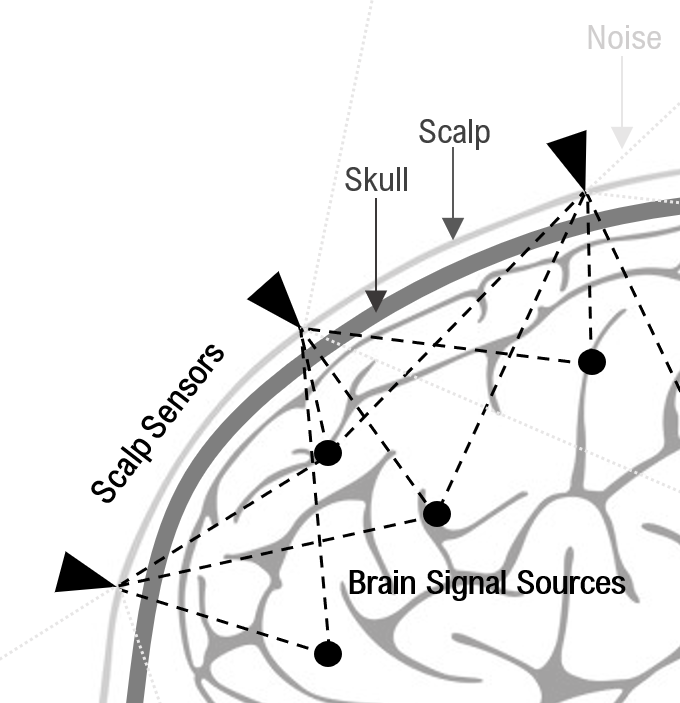
\includegraphics[width=\textwidth]{figures/EEG/volumeconduction.png}
        \caption{Illustration of volume conduction.}\label{fig:volumeconduction}
    \end{minipage} 
    \hfill
    \begin{minipage}[t]{.45\textwidth}
        \centering
        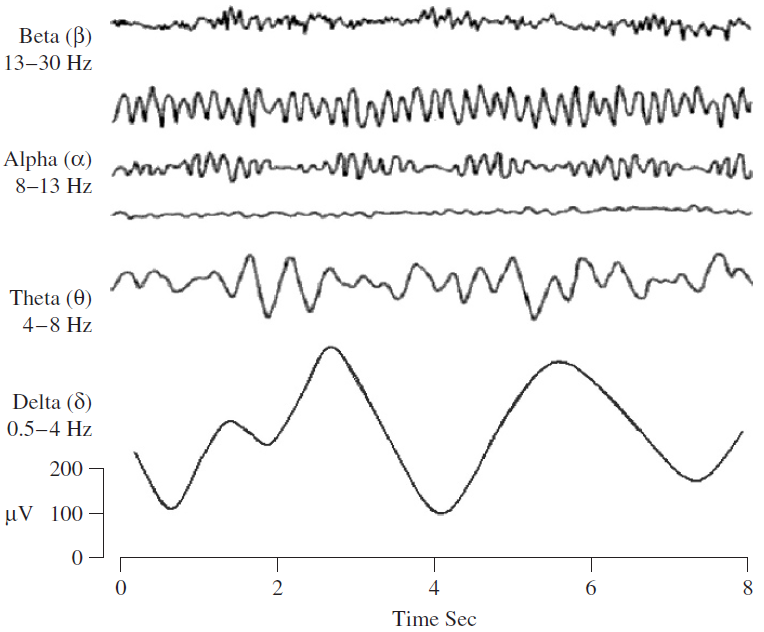
\includegraphics[width=\textwidth]{figures/EEG/EEG_example.png}
        \caption{Example of time dependent signals within the four defined categories \cite{EEGsignalprocessing}.}\label{fig:EEG_example}
    \end{minipage}
\end{figure}
\noindent

\subsection{Applications}\label{seg:application}
EEG performed on humans and animals have a great number of applications within both clinical and research purposes. 
Examples of clinical applications covers diagnosis and management of neurological disorders like epilepsy, and monitor alertness regarding coma or brain death.
EEG capitalizes on the procedure being non-invasive and fast.
Neural activity can be measured within fractions of a second after a stimulus has been provided. 
These advantages contribute to the wide range of applications within research of the neural processes involved in or resulting from actions, emotions or cognition. Today such neural research are used in many different fields \cite[p. 4]{fundamentalEEG}.
The hearing aid industry is one example where this research is highly prioritized. 
At Eriksholm research center, which is a part of the hearing aid manufacturer Oticon, cognitive hearing science is a research area within fast development \cite{Weberik}. 
One main purpose at Eriksholm is to make it possible for a hearing aid to identify the user-intended sound source from real-time EEG measurements and thereby exclude noise from elsewhere \cite{Emina2019}\cite{Bech2018}. 
It is essentially the well-known but unsolved cocktail problem which is sought improved by use of EEG. 
This is where EEG and occasionally so called in-ear EEG is interesting. In conjunction with the technology of beamforming, it is possible for a hearing aid to receive only signals from a specific direction. 

Over the past two decades functional integration has become an area of interest regarding EEG research \cite{Friston2011}. 
Within neurobiology functional integration refers to the study of the correlation among activities in different regions of the brain. 
In other words, how do different parts of the brain work together to process information and conduct a response \cite{Friston2002}. 
For this purpose recovery of the original source signals, from EEG measurements, is of interest. 
An article from 2016 \cite{Van2019} points out the importance of performing analysis regarding functional integration on the sources, rather than directly on the EEG measurements. This relation is referred to source level versus EEG level. 
It is argued through experiments that analysis at EEG level does not allow interpretations about the interaction between sources. 
This emphasizes a potential for improving results within a wide range of EEG research, if the original source signals can be recovered from an EEG measurement.    

%     
%However, the focus of this research is the correlation between EEG measurements and the sound source rather than localization of the activated source from the EEG \cite{Emina2019}. 
%Hence a source localization approach could potentially be of interest regarding hearing aids in order to improve the results.
%(Furthermore, a real-time application to provide feedback from EEG measurements would be essential.)\todo{?}. 


\subsection{Modeling}
Consider the issue of recovering the source signals from EEG measurements. A known approach is to model the observed measurements by a linear system 
\begin{align*}
\mathbf{y} = \mathbf{Ax}.
\end{align*}
Let the vector $\mathbf{y} \in \mathbb{R}^{M}$ be the EEG measurements of one time sample containing $M$ sensor measurements. Let $\mathbf{x} \in \mathbb{R}^{N}$ be the corresponding $N$ sources within the brain. 
Non-zero entries of $\textbf{x}$ represent the active sources at the time of the measurement. 
Then the matrix $\mathbf{A} \in \mathbb{R}^{M \times N}$ represents the linear transformation from $\mathbb{R}^{N}$ to $\mathbb{R}^{M}$. The matrix $\mathbf{A}$ will be referred to as the mixing matrix as it resembles the volume conduction. 
The $j$-th column of $\mathbf{A}$ represents the relative weights from the $i$-th source to every sensor \cite{phd2015}. 
Representing one time sample the linear system is in general referred to as a single measurement vector model. 
Only the measurement vector $\mathbf{y}$ is known, hence it is impossible to solve the linear system with respect to $\mathbf{x}$ using basic linear algebra. 
The task, in this case, is to recover first $\mathbf{A}$ and then $\mathbf{x}$, given the measurement vector $\mathbf{y}$. This problem is referred to as the inverse EEG problem. 
Recovering $\mathbf{x}$ by some estimate $\hat{\mathbf{x}}$ is referred to as source identification and localization. Identification is to estimate the signal of each active source. Localization is to place each active source signal at the right position within the source vector of dimension $N$, where $N$ is the maximum number of sources.      

\subsection{Solution Method}\label{sec:ICAsolution}
Independent Component Analysis (ICA) is one commonly applied method to solve the inverse EEG problem \cite{Scott1996}\cite{Scott1997}. ICA is a technique to find the mixing matrix $\mathbf{A}$ such that the rows of $\mathbf{x}$ is statistically independent. 
Thus statistical independence between the sources is a necessary assumption. With respect to the nature of EEG measurements, this assumption is considered valid \cite[p. 3]{Scott1997}. 
Application of ICA has shown great results regarding source recovery from EEG measurements. 
However, a significant flaw to this method is that the EEG measurements are only separated into the number of sources equal to or less than the number of sensors \cite{Balkan2015}.
Meaning that the inverse EEG problem can not be solved in the case where the maximum number of sources $N$ exceeds the number of sensors $M$ -- the model forms an under-determined system. 
Such limitation undermines the reliability and usability of ICA, as the number of active sources easily exceeds the number of sensors \cite{phd2015}. 
This is especially a drawback when low-density EEG is considered. Low-density EEG measurements are collected from equipment with less than 32 sensors, increasing the changes for the number of sources to exceed the number of sensors. 
However, the improved capabilities of low-density EEG devices are desirable due to their relative low cost, mobility and ease to use. 
Especially within the hearing aid industry, as mentioned earlier, where low-density EEG equipment can be combined with a hearing aid.  

This argues the importance of considering the inverse problem of EEG in the under-determined case where $M < N$. In the following section existing work considering the under-determined inverse EEG problem is investigated further. 

\section{Related Work and Our Objective}\label{sec:relatedwork}
As mentioned above ICA is a solid method for source identification in the case where separation into a number of sources equal to the number of sensors is adequate. The issue occurs in cases where the number of sources $N$ exceeds the number of sensors $M$. 
To overcome this issue, an extension of ICA was suggested, referred to as the ICA mixture model \cite{Balkan2015}.
Instead of identifying one mixing matrix $\mathbf{A} \in \mathbb{R}^{M \times N}$ from an under-determined system this approach learns $N_{\text{model}}$ different mixing matrices $\mathbf{A}_i \in \mathbb{R}^{M\times M}$, to make computations more tractable. 
This method was further adapted into the Adaptive Mixture ICA (AMICA) which has showed successful results regarding identification of more sources than sensors \cite{Palmer2008}. 
However, these successful results rely on the assumption that no more than $M$ out of $N$ possible sources is simultaneously active. That is explicit that the source vector of dimension $N$ has at most $M$ non-zero entries.
This assumption is still an essential limitation to the framework, especially when considering low-density EEG. 
Other types of ICA algorithms for under-determined systems were proposed, without overcoming the limitation of jointly active sources exceeding the number of sensors.
%One is the Restricted ICA (RICA), an efficient method used for unsupervised learning in neural networks \cite{Le2011}.\\ 

In 2015 O. Balkan et. al. suggested a new approach targeting the identification of more active sources than sensors regarding EEG measurements. One method was proposed for learning the mixing matrix $\mathbf{A}$ from measurements $\mathbf{y}$ \cite{Balkan2015} and a different method was proposed for finding the source signals $\mathbf{x}$ given $\mathbf{y}$ and $\mathbf{A}$ \cite{Balkan2014}.

To learn $\mathbf{A}$ the suggested method, referred to as Cov-DL, is a covariance-domain based dictionary learning algorithm. 
The method is based upon theory of dictionary learning and compressive sensing. Which dictates a framework for solving an under-determined system when $\mathbf{x}$ contains a sufficiently amount of zeros. 
This is similar to the constraint of the presented ICA methods. However, to overcome this, the point of Cov-DL is to transfer the EEG measurements into the covariance-domain. In the covariance-domain a higher dimensionality can be achieved compared to the original EEG sensor domain with dimension $M$.
The transformation can be done under already discussed assumptions of linear mixing and uncorrelated sources which follows from the assumption of independence.
As a result the theory of compressive sensing is found to apply successfully to the covariance-domain, allowing to learn $\mathbf{A}$ by dictionary learning. Even in the case where the active sources exceed the number of sensors.

Thus, the Cov-DL method stands out from other straight forward dictionary learning methods as it does not relay on the sparsity of active sources. Where sparseness refers to the number of non-zero elements. This is an essential advantage when low-density EEG is considered. 
Cov-DL was tested and found to outperform AMICA \cite{Balkan2015}. 
As mentioned, the Cov-DL method only learns the mixing matrix $\mathbf{A}$, resembling the volume conduction.

For the purpose of recovering $\mathbf{x}$, from $\mathbf{y}$ and $\mathbf{A}$, a multiple measurement sparse Bayesian learning (M-SBL) method is proposed \cite{Balkan2014}. M-SBL is based on the concept of finding a set of non-zero indices of the source vector $\mathbf{x}$ which corresponds to finding the localization of sources. Followed by an identification of each source signal. The method builds upon the Bayesian statistic framework and it is targeting the case of more active sources than sensors.
The method was proven to outperform the previously used algorithms, even when the defined recovery conditions regarding the found mixing matrix $\mathbf{A}$ was not fulfilled \cite{Balkan2014}.

One drawback, which is not fully covered in the referred literature, is the two methods rely on the number of active sources being known. 
In practice this is not the case. 
Hence, an estimation of the number of active sources has to be considered for the methods to be useful in practice.

The two state of the art methods resulting in source recovery will make the foundation of this thesis. 
Our aim is to investigate and fully understand the two methods in order to implement and test a joint algorithm. The recovering the original source signals $\mathbf{x}$ from the measurements $\mathbf{y}$, when the number of active sources exceeds the number of measurements. More specifically the goal is to support the current results, by applying the methods on different EEG measurements, through our own implementation of the methods into one algorithm. 
Secondary it is of interest to consider the practical application of the proposed algorithm, for instance within a hearing aid as described in section \ref{sec:EEG}. 
%As described in section \ref{sec:EEG} it is of interest to reduce the amount of energy it takes to listen to a specific sound source surrounded by noise.
%For this purpose we want to relate the found number of active sources to the level of concentration that the test person is experiencing. 
As mentioned, the number of active sources is in general unknown in practice.
Thus, an estimation of the number of active sources is of interest for practical use of the algorithm. 
For this we want to investigate whether it is possible to estimate the number of active sources based on the recovered source signals. 

By figure \ref{fig:problem} the presented problem of source signal recovery from EEG measurements is considered within the bigger context which has been discussed in this chapter. Leading from the possibilities of EEG measurements to the specific application within hearing aids, as mentions above.    
\begin{figure}[H]
\centering
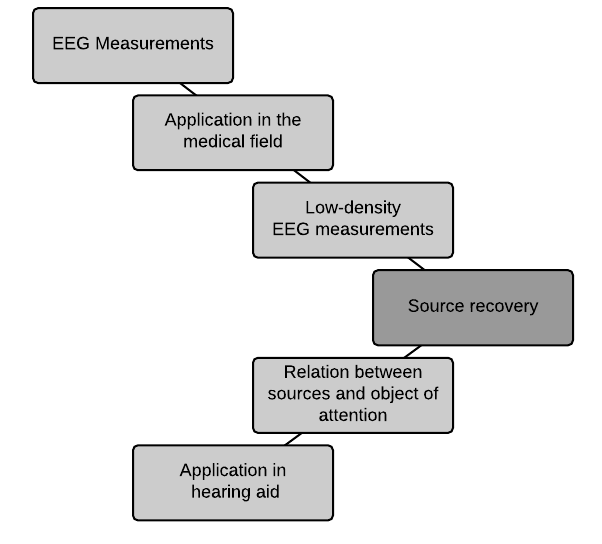
\includegraphics[scale=0.85]{figures/ch_intro/system.png}
\caption{Visualization of the specified issue of source signal recovery relative to a bigger context.}
\label{fig:problem}
\end{figure}
\noindent




